\chapter{Simulation Results}
\section{Model Predictive Controller}
Due to the pendulums setup, the MPC formulation (\ref{mpcgeneral}) could be applied directly. As known, a linear MPC uses a linear prediction model of the process to predict the behavior of the system over the prediction horizon. So such a predictive controller is used to control the pendulum in range, where such a linear predictive model is relevant.So the first step of the construction of such a controller is to obtain the discrete-time linear predictive model via discretization of (\ref{linmatrices}) at the upright operation point 
\begin{equation}
	\ui{x}{up} = \begin{bmatrix}0,0,0,0\end{bmatrix}^\intercal, 
\end{equation}
with the discretization step $0.02$, what is equal to real devices sampling time. 
\begin{subequations}\label{dismatrices}
	\begin{align}
	\ui{A}{D} &=\begin{bmatrix}
	1&0.02&-0.0031& 0\\
	0&1&-0.3140&-0.0031\\
	0&0&\ \; \,1.0161&\ \; \,0.0201\\
	0&0&\ \; \,1.6096&\ \; \,1.0161
	\end{bmatrix}\\
	\ui{B}{D} &=\begin{bmatrix}
	\ \; \,0.0035\\
	\ \; \,0.3509\\
	-0.0081\\
	-0.8083
	\end{bmatrix}\\
	\ui{C}{D} &= \begin{bmatrix}0&0&1&0\end{bmatrix}\\
	\ui{D}{D} &= 0
	\end{align}
\end{subequations}
The next step is to design weight matrices $\ui{Q}{x}$ and $\ui{Q}{u}$.
\begin{equation}
\ui{Q}{x} = \begin{bmatrix}
1.5&0&0&0\\
0&0.08&0&0\\
0&0&10&0\\
0&0&0&0.2
\end{bmatrix}, \quad \ui{Q}{u} = 1
\end{equation}
The main weights are given obviously to the position of the pendulum, what is our main controlled parameter, and the position of the arm, to prevent the possible scenario when the pendulum is stabilized at the upright position and the arm rotates constantly. 
The remain MPC parametres are shown in the following table
\begin{table}[h]
	\caption{MPC parameters during the stabilization at the upright position}
	\begin{tabular}{l c c}
		\noalign{\hrule height 1pt}
		Parameter&Symbol&Value\\
		\hline
		Prediction horizon&$N$&$20$\\
		Initial condition&$x_0$&$\begin{bmatrix}-1,-2,0.5,2\end{bmatrix}^\intercal$\\
		Constraint on control input-upper bound&$\ui{u}{max}$&$\ \; \,5$\\
		Constraint on control input-lower bound&$\ui{u}{min}$&$-5$\\
		\noalign{\hrule height 1pt}
	\end{tabular}
\end{table}
\newpage
\begin{figure}[H]
	\centering
	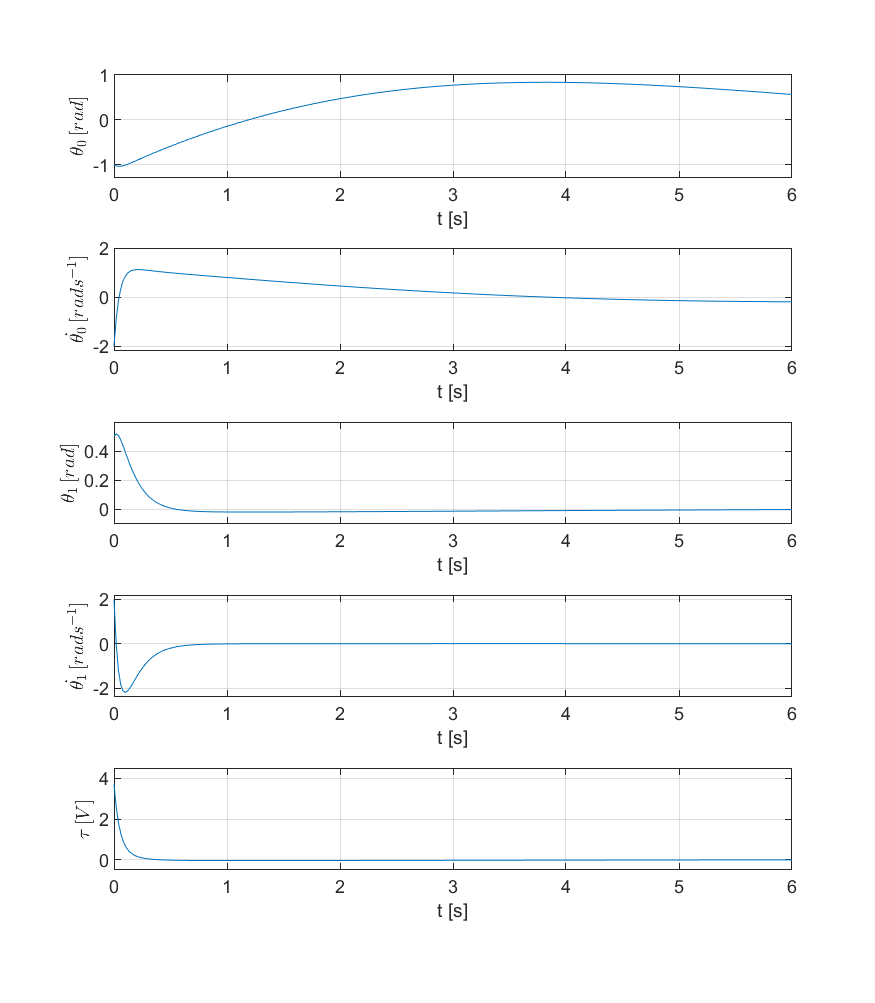
\includegraphics[width=1.1\linewidth]{images/MPC}
	\caption{Simulation results for a scenario with stabilization at the upright position by linear MPC. The plots depict, respectively, the individual states , the third of which is the controlled pendulum position $\theta_1(t)$, and the control input $\tau(t)$.}
	\label{mpc}
\end{figure}
\newpage
\section{Energy-Shaping Controller}
The main purpose of the Energy-Shaping controller is to swing the pendulum from the downside position into the upright position where the control of the process will be taken by another controller. 
Such controller can be designed by applying the control law (\ref{energy-shaping}) directly as a state-feedback controller.
\newpage
\begin{figure}[H]
	\centering
	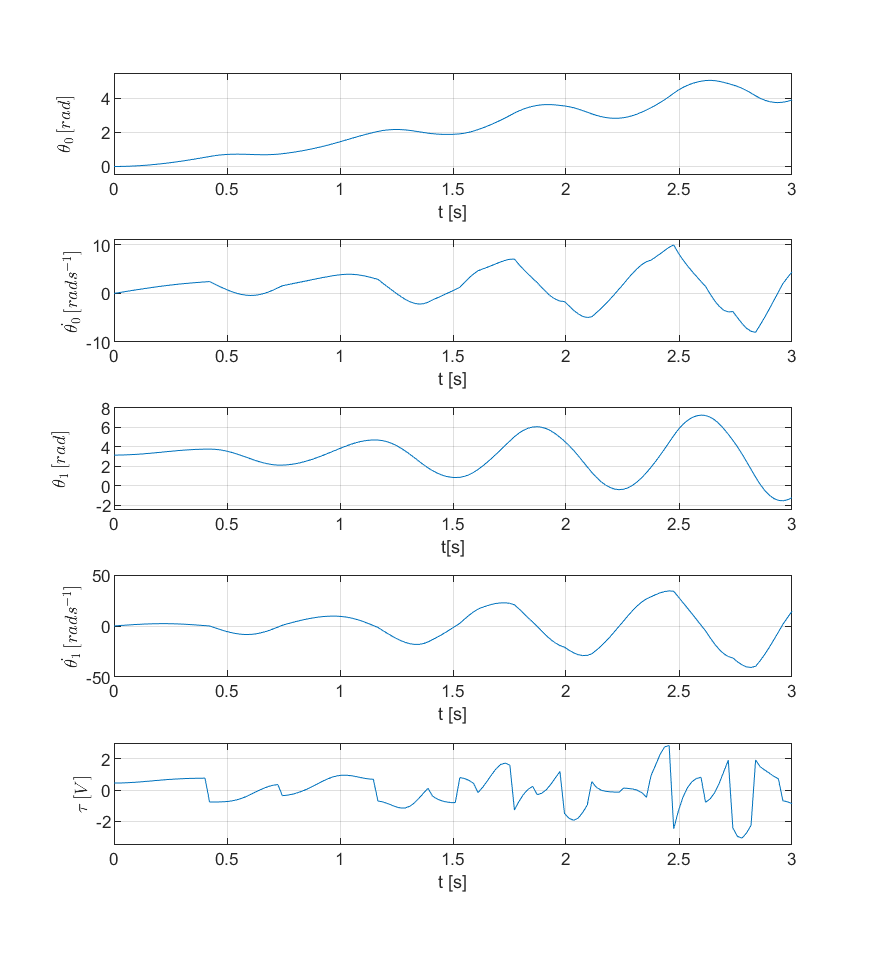
\includegraphics[width=1.1\linewidth]{images/Swing}
	\caption{Initial oscillation of the system by the Energy-Shaping controller. The plots depict, respectively, the individual states , the third of which is the controlled pendulum position $\theta_1(t)$, and the control input $\tau(t)$.}
	\label{swing}
\end{figure}
\newpage
\section{Heuristic Swing-Up Control}
To perform Swing-Up Control of the pendulum, a combined control strategy should be designed, because no MPC nor Swing-Up controller can not perform a Swing-Up control by itself. So the strategy of Heuristic Swing-Up Control is that at the beginning the pendulum is steady at the downside position and the Energy-Shaping controller is used to add the energy to the pendulum via its oscillation. As more energy is added to the pendulum, the greater the oscillations become. As the pendulum is close to the upright operation point, the control law switches from Energy-Shaping to MPC. And MPC finishes the Swing-Up Control by stabilizing the pendulum at the upright position.
\newpage
\begin{figure}[H]
	\centering
	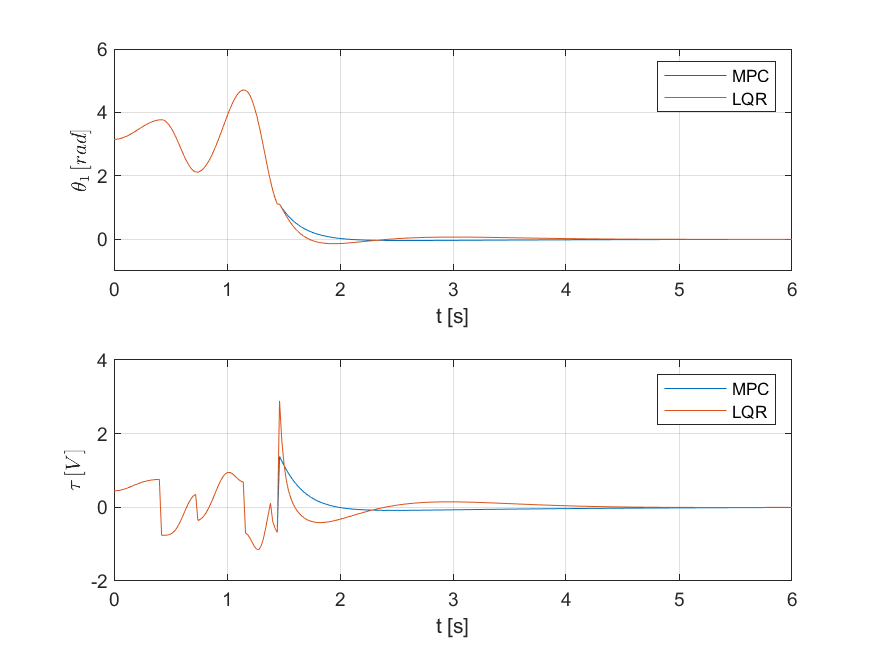
\includegraphics[width=1.1\linewidth]{images/MPC-LQR_Swing}
	\caption{Simulation result of the Swing-up control of the pendulum by Energy-Shaping+Mpc combined control strategy. The first plot depict the controlled pendulum position $\theta_1(t)$, and the second - control input $\tau(t)$.}
	\label{combo}
\end{figure}
\newpage
\section{NMPC}
To design a Nnlinear Model Predictive Controller freely availabe \textit{MATMPC} toolbox is used. This toolbox which could be downloaded from \textit{https://github.com/chenyutao36/MATMPC}. Also additional software is required:
\begin{itemize}
	\item \textbf{CasAdi} - the state-of-the-art automatic/algorithmic differentiation toolbox.
	\item \textbf{MinGW-w64 C/C++ Compiler} - algorithmic routines are compiled
	into MEX functions using this compiler.
\end{itemize}
Basically \tt{MATMPC} solves the folloving NLP problem:
\begin{subequations}\label{NLP}
	\begin{align}
	\min_{U} &\sum_{k=0}^{N-1} (\left\| \ui{Q}{x}x_{k}\right\|_p+\left\|\ui{Q}{u}u_{k}\right\|_p)\\
	s.t.\quad&x_{k+1} = \phi(x_{k},u_{k})\qquad k \in \mathbb{N}_0^{N-1}\\
	&x_0 = x(t)\\
	&x_{k}\in\mathcal{X}\qquad\qquad\qquad\!\: k \in \mathbb{N}_0^{N-1}\\
	&u_{k}\in\mathcal{U}\qquad\qquad\qquad\, k \in \mathbb{N}_0^{N-1}
	\end{align}
\end{subequations}
where $\phi(x_{t+k},u_{t+k})$ is a numerical integration operator that solves the following initial value problem (IVP) and returns the solution at $t_{k+1}$.
\begin{equation}
0=\ui{f}{impl}\lrp{\dot{x}(t), x(t),u(t),t},\quad x(0)=x_k.
\end{equation}
To obtain a numerical solution to that NLP problim \tt{MATMPC} uses a SQP strategy to construct and solve a sequence of following quadratic problems
\begin{equation}\label{QP}
\begin{aligned}
\min_{\Delta \mathbf{x},\Delta \mathbf{u}} \quad & \sum_{k=0}^{N-1}( \frac{1}{2}
\begin{bmatrix}
\Delta x_k\\
\Delta u_k
\end{bmatrix}^\intercal \begin{bmatrix}
Q_k^i & S_k^i \\
S_k^{i^\top} & R_k^i
\end{bmatrix}
\begin{bmatrix}
\Delta x_k\\
\Delta u_k
\end{bmatrix} + \begin{bmatrix}
g_{x_k}^i\\
g_{u_k}^i
\end{bmatrix}^\intercal
\begin{bmatrix}
\Delta x_k\\
\Delta u_k
\end{bmatrix} ) \\
s.t. \quad & \Delta x_0=\hat{x}_0-x_0\\
& \Delta x_{k+1}=A_{k}^i \Delta x_{k}+ B_{k}^i \Delta u_{k} +a_{k}^i \qquad k \in \mathbb{N}_0^{N-1}\\
& \Delta x_{min}\leq \Delta x_k\leq \Delta x_{max}\qquad\qquad\quad\; k \in \mathbb{N}_1^{N}\\
& \Delta u_{min}\leq \Delta u_k\leq\Delta u_{max}\qquad\qquad\quad\; k \in \mathbb{N}_0^{N-1}\\
\end{aligned}
\end{equation}
where 
\begin{equation}
\begin{aligned}
&\Delta \mathbf{x}=\mathbf{x}-\mathbf{x}^i\\
&\Delta \mathbf{u}=\mathbf{u}-\mathbf{u}^i
\end{aligned}
\end{equation}
and
\begin{equation}\label{QP data}
\begin{aligned}
&g_{x_k}^i = \frac{\partial d^i}{\partial x_k},\quad g_{u_k}^i = \frac{\partial d^i}{\partial u_k},\\
&A_k^i=\frac{\partial \phi_k}{\partial x_k}, \quad B_k^i=\frac{\partial \phi_k}{\partial u_k},\quad a_k^i = \phi(x_k^i,u_k^i)-x_{k+1}^i,\\
\end{aligned}
\end{equation}
Where outer objective function $d:\mathbb{R}^{n_y}\rightarrow \mathbb{R}$, is convex. The Hessian matrices $Q_k,S_k,R_k$ can be approximated by the Gauss-Newton (GN) or the Generalized-Gauss-Newton (GGN) method. By solving that QP the optimal primal solution $(\Delta \mathbf{x}^{i^*}, \Delta \mathbf{u}^{i^*})$ is obtained. That primal solution is used to update the solution of \eqref{NLP} by
\begin{subequations}
	\begin{align}
	\mathbf{x}^{i+1} = \mathbf{x}^{i} + \alpha^i \Delta\mathbf{x}^{i^*}, \\ \mathbf{u}^{i+1} = \mathbf{u}^{i} + \alpha^i \Delta\mathbf{u}^{i^*},
	\end{align}
\end{subequations}
where $\alpha^i$ is the step length determined by globalization strategies. 
Now only weight matrices $Q_x$ and $Q_u$ remain:
\begin{equation}
	\ui{Q}{x} = \begin{bmatrix}
	1&0&0&0\\
	0&0.1&0&0\\
	0&0&2&0\\
	0&0&0&0.1
	\end{bmatrix} \quad \ui{Q}{u} = 0.1
\end{equation}
And now with such setup, a swing-up control of the Furuta Pendulum is performed
\newpage
\begin{figure}[H]
	\centering
	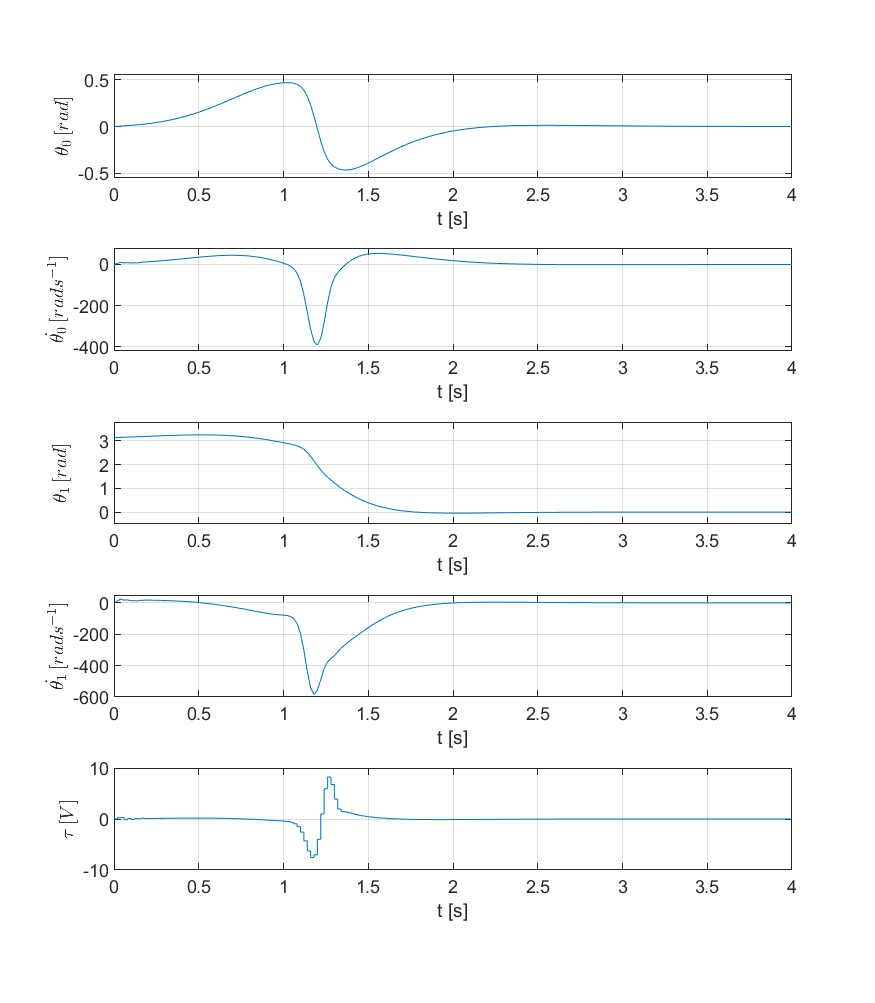
\includegraphics[width=1.1\linewidth]{images/NMPC}
	\caption{Simulation result of the Swing-up control of the pendulum by NMPC strategy.The plots depict, respectively, the individual states , the third of which is the controlled pendulum position $\theta_1(t)$, and the control input $\tau(t)$.}
	\label{NMPC}
\end{figure}